\documentclass[letterpaper,10pt]{article}

\usepackage{titling}
\usepackage{listings}
\usepackage{url}
\usepackage{setspace}
\usepackage{subfig}
\usepackage{sectsty}
\usepackage{pdfpages}
\usepackage{colortbl}
\usepackage{multirow}
\usepackage{multicol}
\usepackage{relsize}
\usepackage{amsmath}
\usepackage{wasysym}
\usepackage{fancyvrb}
\usepackage{amssymb}
\usepackage{ifsym}
\usepackage{amsmath,amssymb,amsthm,graphicx,xspace}
\usepackage[titlenotnumbered,noend,noline]{algorithm2e}
\usepackage[compact]{titlesec}
\usepackage{XCharter}
\usepackage[T1]{fontenc}
\usepackage{tikz}
\usetikzlibrary{arrows,automata,shapes,trees,matrix,chains,scopes,positioning,calc}
\tikzstyle{block} = [rectangle, draw, fill=blue!20, 
    text width=2.5em, text centered, rounded corners, minimum height=2em]
\tikzstyle{bw} = [rectangle, draw, fill=blue!20, 
    text width=4em, text centered, rounded corners, minimum height=2em]

\definecolor{namerow}{cmyk}{.40,.40,.40,.40}
\definecolor{namecol}{cmyk}{.40,.40,.40,.40}

\let\LaTeXtitle\title
\renewcommand{\title}[1]{\LaTeXtitle{\textsf{#1}}}


\newcommand{\handout}[5]{
  \noindent
  \begin{center}
  \framebox{
    \vbox{
      \hbox to 5.78in { {\bf ECE356: Database Systems } \hfill #2 }
      \vspace{4mm}
      \hbox to 5.78in { {\Large \hfill #4  \hfill} }
      \vspace{2mm}
      \hbox to 5.78in { {\em #3 \hfill} }
    }
  }
  \end{center}
  \vspace*{4mm}
}

\newcommand{\lecture}[3]{\handout{#1}{#2}{#3}{Lecture #1}}
\newcommand{\tuple}[1]{\ensuremath{\left\langle #1 \right\rangle}\xspace}

\addtolength{\oddsidemargin}{-1.000in}
\addtolength{\evensidemargin}{-0.500in}
\addtolength{\textwidth}{2.0in}
\addtolength{\topmargin}{-1.000in}
\addtolength{\textheight}{1.75in}
\addtolength{\parskip}{\baselineskip}
\setlength{\parindent}{0in}
\renewcommand{\baselinestretch}{1.5}
\newcommand{\term}{Winter 2018}

\singlespace


\begin{document}

\lecture{ 32 --- Distributed Databases }{\term}{Jeff Zarnett}

\section*{Distributed Databases}

A distributed database is basically a scaled up shared nothing system. The database is stored on multiple computers and almost always at multiple physical locations. The systems that make up the distributed database need not be the same (e.g., they may have different CPU types, different amounts of memory, different operating systems, etc). This is probably out of necessity: you can't order a computer with 4000 CPUs and and 64~000 GB of RAM and 2000 hard drives, right? But you can order a thousand computers that each have 4 CPUS, that have 64 GB of RAM and 2 hard drives.

Our discussion of distributed databases is not in any sense a replacement for a distributed systems course but it might be a bit of an introduction to the topic that might increase your interest in it. 


\subsection*{Transparency}
When designing a distributed system one of the primary concerns is \textit{transparency}, but not the sort we expect of governments where we should know what is going on. It's actually the opposite: what we want is for it to be imperceptible to the users that the database is distributed. There are a few types of transparency that are possible (and generally they are desirable nut not necessarily)~\cite{fds}:

\begin{itemize}
	\item \textbf{Location Transparency}: The command used to perform a task is the same no matter the node on which it executes.
	\item \textbf{Naming Transparency}: When an item has a name, it can be accessed via the name regardless of location.
	\item \textbf{Replication Transparency}: Copies of the data can be stored in multiple locations for reasons such as performance, availability, or reliability. The user should not be aware that the data is a copy (which implies the copies need to agree... or at least not contradict each other).
	\item \textbf{Fragmentation Transparency}: The database can be broken up into multiple parts and it means a query may need to be broken up into multiple subqueries and recombined without noticing. 
\end{itemize}

\subsection*{Fragmentation}

Fragmentation is splitting up data. A relation $r$ can be divided up into arbitrarily many fragments $r_{1}, r_{2}, ..., r_{n}$; combining all the fragments again will allow reconstruction of the original relation $r$. 

\paragraph{Horizontal Fragmentation.} In horizontal fragmentation, each part of the relation $r_{i}$ contains some number of complete tuples. Each tuple is assigned to one or more fragments (but it has to be in at least one of them). If we were looking at a bank that had data centres in, say, New York and Hong Kong, then the tuples of the account data for the New York customers would be located in the New York data centre and the HK ones in HK. This keeps tuples close to where they are used the most, to minimize the data transfer requirements; it does not mean that the tuples are inaccessible at other locations; they are just going to take longer to retrieve~\cite{dsc}.

If it helps with understanding, the definition of the table is the same at both locations, but some rows are in one database and some in the other.

In relational algebra representation, a fragment $r_{i}$ is created by a selection with a predicate. So a fragment $r_{i} = \sigma_{P_{i}}(r)$ and the entire relation can be reconstructed as a union of the sets~\cite{dsc}. This works only if the sets are disjoint -- no tuples are duplicated. If we have non-disjoint fragments then we might have the possibility of duplicate data, so we would need some sort of de-duplication to produce $r$ again in a consistent way.

\textit{Derived horizontal fragmentation} applies the partitioning of a relation rules to some secondary tables that are related by a foreign key~\cite{fds}. Imagine you have a relation that is a shipment and there is a related relation of containers. Some number of containers are associated with the shipment (in the logic of the application); it would therefore make sense to split up the container relation based on their relationship to the shipment relation... If a shipment is at location 1, its associated containers should also be at that location.

\paragraph{Vertical Fragmentation.} Vertical integration is splitting up by attributes rather than tuples. 

In relational algebra fragmentation is done using projection: $r_{i} = \Pi_{R_{i}}
(r)$ and they are recombined using the natural join~\cite{dsc}.  For recombination to work, of course, we need a key in each part of the relation. If there are no attributes in common we have no way of recombining. Thus, at least some of the data will be repeated in the various partitions. In horizontal fragmentation the sets can be completely disjoint, but that is not the case in vertical fragmentation. 

Now, the tables have different definitions -- and there are some columns for each row in one database and some in the other. 


\paragraph{Hybrid (Mixed) Fragmentation.} This is the all-of-the-above sort of fragmentation, where both horizontal and vertical fragmentation are applied. Recombination of the relation is accomplished by performing the union and outer join operations in the appropriate order~\cite{fds}. 

\subsection*{Replication}

Replication is making copies of the data available in different database servers. This may be to improve availability or reliability of data. At the one extreme, all data is replicated to all sites in the distributed system, meaning every location has all the data. This has its advantages and disadvantages, as we'll examine. 

The simplest way to replicate is to not do it at all: there are no duplicate copies of the data and whatever fragment is at each location is the only copy. This means to get the full data, all systems must be online and available. 

If we do choose to replicate all of the data, then this is a fully-replicated distributed database. The system can continue to function as long as any one location is operational, and it can improve performance of retrieval of data since we can always query the closest database~\cite{fds}. Unfortunately it means much more work on an update since all locations have to be updated. In fact, getting everyone to agree on what happened (or didn't) is a problem that is big enough to have its own minor topic. 

In between is partial replication: some data is replicated over multiple sites and or all data is replicated in some way (e.g., any one piece of data is on at least three servers but may not be on all servers). A special case is when mobile workers go out into the field in areas where there is no internet connection, carrying a copy of the database, and have to synchronize when they get WiFi with some central server(s)~\cite{fds}.

Wherever data is replicated, we can choose one of the replicas to be the primary copy~\cite{dsc}. If the whole database is replicated then one database site is the primary site and has the primary copy of all the data. 

In databases under heavy load, replication is one of the keys to improving performance. A very common strategy is for reads to be done on replicas, with one database designated as the write master and all writes are done on the write master. The changes are then propagated to all replicas once the write is completed. This improves performance because we avoid the two problems we are going to talk about next: distributed locking and distributed transaction management.

\subsection*{Distributed Locking}

If we take the single lock manager approach, there is one single lock manager and one site is chosen as the leader. All requests are sent to that one site and that system tells the other system whether the request is granted, denied, or delayed. A read can be done at any one site that has the data, but a write requires all sites that have that data to participate~\cite{dsc}.

The single lock manager approach is simple in that there are only requests and responses and everything is managed centrally so there is no need to invest effort to make sure that different lock managers agree. But there is the risk of failure at this one location causing the whole system to stop or misbehave.

If we choose instead to let all sites be involved in lock management, we have distributed lock management and the function is distributed. Immediately we can imagine this introduces the possibility that a disagreement arises about what data is locked and whether a lock can be granted. But it does mean that we no longer are constrained by the single site. We do have ways of handling the complexity.

\paragraph{Primary Copy.}A simple approach to distributed locking is using the primary copy as controlling: if a site wishes to lock an item, it has to acquire the lock at the primary site. Thus, each site is responsible for keeping control over the data it is the primary for. The obvious downside is that if a site goes down, the data for which it is the primary is inaccessible even though there is a replica of it (until some other site takes over primary ownership)~\cite{dsc}.

\paragraph{Majority Rules.} The next level up is to use a majority protocol: if a data item $i$ is at $n$ different sites, then a lock message has to be sent to (at least) $\lceil n/2 \rceil$ locations to lock $i$. If a site finds according to its own local situation that the lock can be granted, it returns a yes answer immediately; otherwise the response is delayed until the lock can be acquired. A transaction on $i$ cannot proceed until a lock has been acquired on a majority of the lock messages~\cite{dsc}.

This routine requires a lot of messages: to lock an item requires $\lceil n/2 \rceil$ outgoing requests and also  $\lceil n/2 \rceil$ responses; to unlock an item then another $\lceil n/2 \rceil$ messages.

There is also the possibility of deadlock in this situation. As you know, this occurs when there is a cycle in the resource requests. A transaction $T_{1}$ requests some item $i_{i}$ and then $i_{2}$ and a transaction $T_{2}$ requests $i_{2}$ then requests $i_{1}$. Under normal circumstances we can just require that data elements have to be requested in some predetermined order (e.g., ascending order), that is to say, with lock ordering. Unfortunately for us, in distributed systems this is not a guarantee. A database can send out a request for $i_{1}$ then $i_{2}$ but because of the vagaries of the network the request for $i_{2}$ might arrive first. So we might need to rearrange some requests upon arrival or restart some operations.

\paragraph{Biased Protocol.} Rather than treating every lock and unlock the same, we could make a distinction on shared vs. exclusive locks. In the biased protocol, to get a shared lock, we just need to request a shared lock on an item from any one site that has a replica of that item. To get an exclusive lock, a lock is requested from all sites that have the item~\cite{dsc}.

If we expect that reads are more frequent than writes (this is very likely) then this is a performance increase. Reading any copy of the data can be done with just two messages, although a write requires $2n$ messages for each site where the data is stored. The request ordering problem is still at issue and the risk of deadlock still exists.

\paragraph{Quorum Consensus Protocol.} In the quorum consensus protocol, every site is assigned a weight (non-negative) and then to perform an operation enough sites need to agree (that is, we must have a quorum). To execute a read, enough sites must agree such that their weights reach some threshold $r$; to execute a write enough sites must agree such that their weights reach a threshold $w$. The values for $r$ and $w$ can be the same or they can be set independently~\cite{dsc}.

Why would we choose sites to have different weights? We might have some sites that are remote and have poor internet connections, thus waiting for them might not be sensible. We may also have sites that have poor reliability, in which case we don't want to count on them to respond. In any case, choosing the values of $r$ and $w$ allow choosing how much agreement we need that locks have been acquired before we are allowed to proceed.

\paragraph{Timestamp Protocol.} In the timestamp protocol, every transaction is assigned a unique timestamp. Systems never agree on what time it is, so to make timestamps are unique, they are concatenated with the site identifier as shown below:

\begin{center}
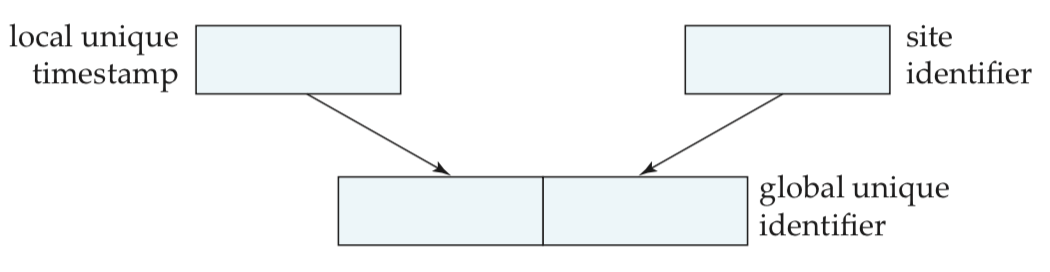
\includegraphics[width=0.5\textwidth]{images/ddb-timestamp}\\
Generating unique timestamps in distributed databases~\cite{dsc}.
\end{center}

The placement of the site identifier in the concatenation is important; if we put it at the beginning then the timestamps at site $k$ would always appear to be after those of $k-1$ and before those of $k+1$, which would not be correct. 

\subsection*{Transaction Management}

In addition to the usual transaction management, there is the global transaction manager that is, more or less, the boss of the other transaction managers. This may be a position where one database server holds the role permanently (it is the boss), or it might be that the database that handles the actual execution, or the one that started it.

Our biggest concern is making sure that everyone agrees. At a fundamental level that means everyone needs to know about the transactions, and needs to agree about whether the transactions are committed or aborted. The first strategy we will examine is the two-phase commit protocol~\cite{fds}. A transaction is sent out to all the participating databases and they will do it.

In phase one, all databases signal the coordinator they are finished with actual execution. When the coordinator has received that from all participating databases, it sends out a message telling all of them to prepare for commit. Then all the databases force write all log records and anything else the recovery process demands to disk. If all goes well they send back a signal saying OK; if something goes wrong they send back a signal that says ``Not OK''. If a timeout is reached without any response then a ``Not OK'' is assumed.

In phase two, if everyone said OK, and the coordinator also says OK, it sends a commit message to all the databases. Every database then proceeds with the commit. If something else happened, then the abort message is sent and all systems roll back the transaction. 

At the end of this, all systems have either committed or aborted the transaction and a consistent state is ensured whether the transaction succeeds or not. If a failure occurs during step one it usually results in rolling back, but if a failure occurs during phase 2 it usually results in commit~\cite{fds}.

This protocol is good but it has some drawbacks. It is a blocking protocol; if the coordinator system fails, all the participating databases end up waiting until the coordinator system is back online. In the meantime they are locking data elements. Alternatively, if a coordinator and participant that have committed crash together, then we might get an indeterminate result~\cite{fds}.

The proposed solution is the three phase locking protocol (MORE PHASES!). The third phase is added in between phase 1 and what previously was phase 2. The new second phase is that the coordinator shares with all participants the results of phase 2. Then phase 3 works just as the commit phase in the two-phase protocol. If the coordinator crashes now, then some other participant can step up and take the coordinator role and see the transaction through. Thus, we can be sure the transaction will finish no matter what system crashes~\cite{fds}. This limits the wait time: based on the phase 1 information we know how the other systems will behave and we can just go ahead and commit; if no such message has been received, abort and proceed with other operations.

\bibliographystyle{alphaurl}
\bibliography{356}


\end{document}
